\documentclass[11pt,english]{article}
\usepackage[T1]{fontenc}
\usepackage{babel}
\usepackage{graphicx}
\usepackage{hyperref}
\usepackage{rotating}
\usepackage{amsfonts}
\usepackage{amssymb}
\usepackage{listings}
\usepackage{color}
\usepackage{amsmath}
\usepackage{titlesec}
\usepackage[linesnumbered, ruled]{algorithm2e}
\usepackage{float}
 
\setcounter{secnumdepth}{4}

\titleformat{\paragraph}
{\normalfont\normalsize\bfseries}{\theparagraph}{1em}{}
\titlespacing*{\paragraph}
{0pt}{3.25ex plus 1ex minus .2ex}{1.5ex plus .2ex}

 
\definecolor{codegreen}{rgb}{0,0.6,0}
\definecolor{codegray}{rgb}{0.5,0.5,0.5}
\definecolor{codepurple}{rgb}{0.58,0,0.82}
\definecolor{backcolour}{rgb}{0.95,0.95,0.92}
 
\lstdefinestyle{mystyle}{
    backgroundcolor=\color{backcolour},   
    commentstyle=\color{codegreen},
    keywordstyle=\color{magenta},
    numberstyle=\tiny\color{codegray},
    stringstyle=\color{codepurple},
    basicstyle=\footnotesize,
    breakatwhitespace=false,         
    breaklines=true,                 
    captionpos=b,                    
    keepspaces=true,                 
    numbers=left,                    
    numbersep=5pt,                  
    showspaces=false,                
    showstringspaces=false,
    showtabs=false,                  
    tabsize=2
}

\lstset{style=mystyle}

\begin{document}
\title{\Huge{\textbf{Deterministic DSA fault attack}}}
\author{
  Fabio Gritti\\
  \texttt{fabio1.gritti@mail.polimi.it}
  \and
  Sebastiano Mariani\\
  \texttt{sebastiano.mariani@mail.polimi.it}
  \and \\
  \textbf{Professors}: Gerardo Pelosi, Alessandro Barenghi
}
\date{}
\maketitle

\pagestyle{plain}
\tableofcontents

\section{Introduction}
In this paper we want to present two active side channel attacks against the deterministic version of the Digital Signature Algorithm ( from now on dDSA ) as specified in the RFC 6979\cite{rfc}.\\
These attacks can lead directly to a leak of the private key and therefore breaking the authenticity of the signatures created using this algorithm. \\\\
We will proceed in this way: first we provide some useful background in order to understand better this paper, then we explain the attacks in details and finally we present the feasibility of the attacks by showing the time needed to break the dDSA with some of the keysize currently available.

\section{Background}

\subsection{The Digital Signature Algorithm}

\subsubsection{General overview}
The DSA is one of three digital signature schemes specified in FIPS 186\cite{fips}. A digital signature scheme is an authentication mechanism that enables the creator of a message to attach a code that acts as a signature providing authenticity and non-repudation. \\It usually consists of three algorithms:

\begin{itemize}
\item a \textit{key generation algorithm} that outputs the private key and the corresponding public key.
\item a \textit{signing algorithm} that given a message and a private key produce the signature. 
\item a \textit{signature verifying algorithm} that given a signature and a public key either accepts or rejects the message's claim to authenticity.
\end{itemize}

In order to be a sound digital signature schemes the following properties must hold:

\begin{itemize} 
\item the authenticity of a signature generated from a given message and a given private key can be verified by using the corresponding public key.
\item it should be computationally unfeasible to generate a valid signature for an user without knowing that users's private key. 
\item The private key MUST remains private, otherwise the authenticity of the signatures created with that key are broken.
\item The public key owner MUST be verifiable, otherwise we can't assure that we had receive a message from a particoular source.
\end{itemize}

\subsubsection{DSA mathematical structure}

The reference group category is $(\mathbb{Z}^{*}_{p},\cdot )$, \textit{p} prime s.t. \textit{q} | ( \textit{p-1} )} with \textit{q} also prime. The employed algebraic structure is then the multiplicative cyclic subgroup \textit{G} = <\textit{g}> with publicly known generator \textit{g} and order \textit{q}.
\\\\
In the FIPS 186-3\cite{fips} standardization the number of bits of the two prime numbers (L = $log_{2}(p)$ N = $log_{2}(q)$ ) are setted to: 1024|160, 2048|224, 2048|256 and 3072|256.

\subsubsection{Cryptoscheme}

Public  Key: $k_{pub} = (p,q,g,g^x)$ \\
Private Key: $k_{priv} = x \in \mathbb{Z}^{*}_{q}$
\\\\
In the following algorithm H stands for an hash function chosen at the beginning of the transformation.

\\

\begin{algorithm}[H]
  \KwData{A message \textit{m} to sign and a dsa key pair}
  \KwResult{The signature of the given message \textit{m} }
  r = 0\;
  s = 0\;
  h = H(\textit{m})\;
  \While{r == 0 or s == 0}{
    k = rand() $\in \mathbb{Z}^{*}_{q}$ \;
    r = $((g^k)$ mod p $)$ mod q \;
    s = $k^{-1} \cdot (H(m) - x \cdot r)$ mod q\; 
  }
  signature = <\texit{r},\textit{s}>\;
  send(m,signature)\;
  \caption{DSA signature transformation algorithm}
\end{algorithm}
\\\\\\
\begin{algorithm}[H]
  \KwData{A DSA signature <\textit{r},\textit{s}> to verify , a message \textit{m} to be verified against the received signature and the dsa public key associated to the private one used to sign the message \textit{m}}
  \KwResult{Accept or not the signature }
  \eIf{r,s $\notin \{1,....,q-1\}$}{
      print "Signature rejected"\;
      return -1\;
    }{
      h = H(\textit{m})\;
      u_{1} = h \cdot $s^{-1}$ mod q \;
      u_{2} = r \cdot $s^{-1}$ mod q \;
      \eIf{($g^{u_{1}}((g^{s})^{u_{2}}$) mod p mod q == r}{
        print "Signature accepted"\;
        return 1\;
      }{
        print "Signature rejected"\;
        return -1\;
      }
   }
  \caption{DSA verify algorithm}
\end{algorithm}

\\\\\\\\

\subsection{The Deterministic Digital Signature Algorithm}

\subsubsection{General overview}
The step in the DSA signing algorithm that requires to generate a random parameter ( a "true" random number, not a pseudorandom one ) needs a great source of randomness in order to be secure; on normal PCs we can generate sound random numbers by exploiting unpredictable data like entropy, the exact time an user press keys on keyboard, the position of the mouse at a specific time, or any other kind of event. \\\\Dealing with embedded systems is a problem from this point of view,in fact we don't have, on board, a real randomness source as before and so not a great RNG to generate unpredictable random numbers for our algorithm! \\This is the crucial point for which many manufacturers decide to employ RSA cryptosystem, that doesn't require random number during the encryption transformation, rather than DSA/ECDSA, the latter in fact require by design a true random number for the encryption transformation.\\
\\The Deterministic DSA proposed in the RFC 6979\cite{rfc} tries to "safely derandomize" the step in the algorithm that needs a true random number for the \textit{k} parameter in order to increase the attractiveness of such system in the embedded world ( smart card, credit card, console or any other kind of board). The security relies on whether the deterministic generation of \textit{k} is indistinguishable from the output of a random oracle.\\\\
Remember that,in any way, we need a good RNG in order to generate a strong private key. 
This proposal make deterministic the signing, NOT the generation of keys that MUST be non deterministic and made a priopri.


\subsubsection{K deterministic generation}

The generation of the deterministic \textit{k} depends only from the message to sign and the private key.\\
According to the RFC, given the input message and a private key, the following process is applied for the generation:

\begin{figure}[H]
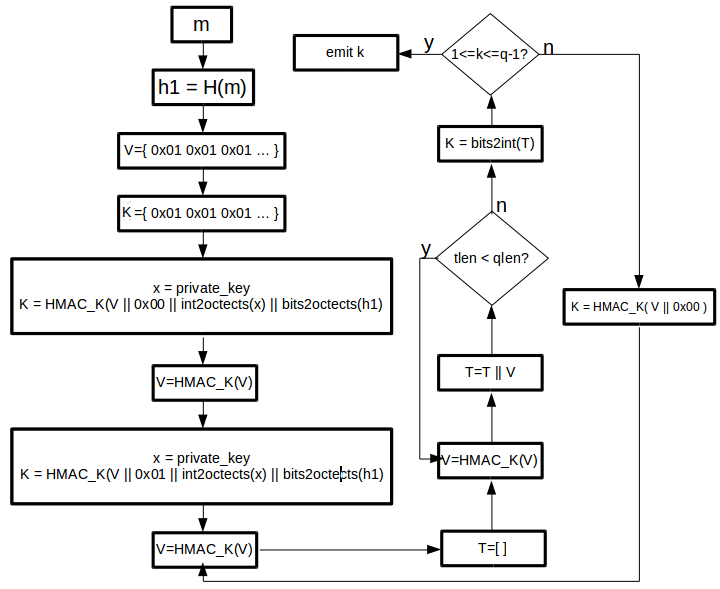
\includegraphics[width=1.0\textwidth]{img/img_2.png} \\
\caption{Generation of deterministic K parameter as specified in the RFC 6979} 
\end{figure}

\begin{itemize}
\item qlen = binary length of the prime number \textit{q}
\item tlen = binary length of the array T 
\item The internal HMAC use the same hash function used in the h1=H(m)
\end{itemize}

This process has been selected in order to maximize as possible the dependency of the deterministic \textit{k} from the message to sign and the private key used. The final goal is to make the deterministic generation of \textit{k} indistinguishable from the output of a random oracle. The math structure behind this is out of scope of this paper, you can read more details in the RFC\cite{rfc}. 

\section{Cracking the Deterministic DSA}

\subsection{Differential fault analysis}

The differential fault analysis is an active side channel attack that is performed in three steps:
\begin{itemize}
\item Obtain the correct signature of a message.
\item Inject a fault during a second signing of the message and obtain the \textit{faulty signature}.
\item Correlate the correct signature with the faulty one and extract the private key.
\end{itemize}

In order to inject a fault we can use different techniques that range from using laser beam during the signing process, to voltage spike or insane overclocking.
\\Usually critical embedded systems like credit card implements different defenses against this fault injection techniques; this raise a lot the cost of an attack performed by an attacker. \\Bypass this kind of defense is out of scope of this paper, our assumption is that the system is vulnerable to this kind of attacks.

\subsection{The attacks}

We test our attacks against the implementation of the RFC 6979\cite{rfc} in the GNU/libgcrypt library\cite{lib}. 
Before start we are going to make a fast briefing about how you can use this library to create digital signature using dDSA. This step is fundamental in order to understand how we simulate the active side-channel attacks via software.\\
The GNU/libgcrypt library\cite{lib} makes heavily use of the so called S-expression\cite{sexp}: a convenient way to parse and store data. For example if we want to generate a dsa key pair we have to write these few lines of code:

\begin{lstlisting}[language=c]

/* gcry_sexp_t is the data type used to store a S-expression */
gcry_sexp_t dsa_key_pair , dsa_parms;

/* 
This function is used in order to build the S-expression 
and store it in dsa_params. These parameters will
tell to the gcry_pk_genkey the options used to generate the key.
*/
gcry_sexp_build(&dsa_parms,NULL,"(genkey(dsa (nbits 4:1024)))");

/*
Finally this is the function that will generate an 
S-expression, stored in dsa_key_pair, that represent 
the dsa key pair.
*/
gcry_pk_genkey(&dsa_key_pair,dsa_parms);
  
\end{lstlisting}

Now that we have a dsa key pair stored in the variable \texttt{dsa\_key\_pair} we can access its field simply:

\begin{lstlisting}[language=c]

/* get the generator of the group employed */
gcry_sexp_t g_param = gcry_sexp_find_token(dsa_key_pair,"g",0);

/* get the prime number 'p' employed */
gcry_sexp_t p_param = gcry_sexp_find_token(dsa_key_pair,"p",0); 

/* get the prime number 'q' employed */
gcry_sexp_t q_param = gcry_sexp_find_token(dsa_key_pair,"q",0);

/* get the private key 'x' */
gcry_sexp_t x_param = gcry_sexp_find_token(dsa_key_pair,"x",0);

/* get the g^x parameter */
gcry_sexp_t y_param = gcry_sexp_find_token(dsa_key_pair,"y",0);

\end{lstlisting}

And signing a message is easy too:

\begin{lstlisting}[language=c]

/* 
let's declare an mpi ( multiple precision number ) in order to 
store the big numerical representation of the message to sign.
*/
gcry_mpi_t msg_digest;

/*
S-expression used in order to declare the plaintext to sign
and receive the ciphertext from the DSA signing algorithm.
*/
gcry_sexp_t ciphertext , plaintext;


/* 
This is the SHA-1 of the message we want to sign. 
in this case: "Hello world."
*/    
const unsigned char* digest = (const unsigned char * )         		"e44f3364019d18a151cab7072b5a40bb5b3e274f";
    
/*
Specific function employed in the library that convert the 
string representation of the message's digest in a multiple 
precision number stored in the  variable 'msg_digest'.
*/    
gcry_mpi_scan(&msg_digest, GCRYMPI_FMT_USG, digest, 
                     strlen((const char*) digest), NULL);

/*
Creation of the S-expression relative to the data to sign.
Here you have to specify the flags rfc6979 in order to 
make use of the deterministic DSA.
You can see this S-expression as the list of options and
parameters for the DSA signing transformation.
*/  
gcry_sexp_build(&plaintext, NULL, "(data (flags rfc6979) (hash %s %b))" , "sha1", 20 , msg_digest);

/*
Start the DSA signing transformation with the options
and parameters passed in the previous step and get
the result in the 'ciphertext' variable.
*/
gcry_pk_sign(&ciphertext, plaintext, dsa_key_pair);

/*
If we want we can also verify here the signature
employing the publickey stored in teh variable
'dsa_key_pair'.
*/
gcry_pk_verify (ciphertext, plaintext, dsa_key_pair);

\end{lstlisting}

We have presented how you can generate and use a pair of dsa key in order to sign a message using the dDSA specified in the RFC\cite{rfc}. \\\\
In order to simulate the attack using the library we added an "attack parameter" (in the next example \textit{attack2}) during the building of the S-expression relative to the parameters of the DSA signing transformation:

\begin{lstlisting}[language=c]
gcry_sexp_build(&ptx2, NULL, "(data (flags rfc6979) (hash %s %b) (attack2))" , "sha1", hash_len , digest);
\end{lstlisting}

We have then modified a bit the library ( specifically the function \textit{dsa-sign} in the file \textit{/libgcrypt/cipher/dsa.c}) in order to redirects the flow to our functions that injects the desidered fault based on the type of the attack we want to perform, we will call this a small "attack dispatcher". In total we added 3 functions:
\begin{itemize}
\item \texttt{fault\_sign()}: when the flow is redirected to this function we trigger the attack 1 that will damage the exponentation ( more details in the next section )
\item \texttt{fault\_sign\_2()}: calling this function we trigger the attack 2 that will damage the signature composition ( more details in the next section )
\item \texttt{fault\_sign\_2\_byte()}: this is a second version of the attack 2
\end{itemize}

If the "attack dispatcher" doesn't find any "attack parameter", the normal sign() function is called and we obtain the correct signature of the message. 

\begin{figure}[H]
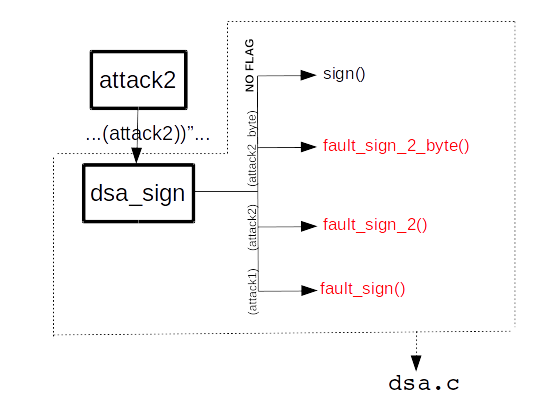
\includegraphics[width=1.0\textwidth]{img/img_3.png} \\
\caption{The schematization of the "attack dispatcher"}
\end{figure}

The next two paragraphs describe the two attacks, then we present the result obtained and finally some limits and considerations.

\subsubsection{Damage the exponentation}

Remembering from the line 6 of the DSA-signing algorithm presented in the section 2.1.3 that we have to exponentiate the generator \textit{g} at the power of the deterministic generated \textit{k}, we injected a bit fault into \textit{k} during the exponentiation, obtaining: g^{\tilde{k}} = \tilde{r} = r \cdot g^{\pm $2^{i}$}. Keep in mind that in the following formula with \textit{m} we indicate the result of H(\textit{m}).

\\\\The attack proceeds as follows:

\begin{itemize}
\item Obtain the correct signature of the message m:  $s = k^{-1}(m + xr) $
\item Obtain the faulty signature of the message m:  $\tilde{s} = k^{-1}(m + x\tilde{r})$
\item Write the system:\\ \\\begin{cases} s \equiv_{q} k^{-1}(m + xr) \\ \tilde{s} \equiv_{q}  k^{-1}(m + x\tilde{r}) \end{cases}\\
\\with \textit{k} and \textit{x} unknown.


\item Solving,we  obtain:\\\\
\begin{cases}
x \equiv_{q} \frac{(s-\tilde{s})m}{(r\tilde{s} - \tilde{r}s)} \\
k \equiv_{q} s^{-1}(mx+r)
\end{cases}

\end{itemize}


This attack is very fast and interesting because in order to calculate the private key \textit{x} we need only the outputs from the two signatures ( the parameters \textit{r} and \textit{s} from the correct one and the parameters \textit{r} and \textit{s} from the faulty one ) and the message \textit{m} passed in plaintext on the channel. The complexity of this attack is basically O(1) since it involves only the resolution of an equation.
\\\\
We checked the attack's correctness by creating a new dsa key pair based on the private key calculated and by signing a new plaintext with that key and then try to verify the signature with the public key of the original dsa key pair.

\subsubsection{Damage the signature composition}

Remembering from the line 7 of the DSA-signing algorithm presented in the section 2.1.3 that we have to perform the multiplication s  = $k^{-1} \cdot (H(m) - x \cdot r)$ mod q , we injected a fault into \textit{k} during this multiplication (in this case before the calculation of $k^{-1}$ , but it would be the same flipping the final result $k^{-1}$ ), obtaining: $\tilde{s} = \tilde{k}^{-1}(m + xr)$.
\\\\
For this attack we have to consider two type of possible injected fault: a bit level fault and a byte level one. The bit level assume that with an active side channel attack we can surgically flip a single bit of \textit{k} during the signature composition, while the byte level is a more realistic assumption that we inject a fault of a whole byte inside the k. Other possible injected fault would be at WORD level,DWORD level, QWORD level, and the more generic fault with different bit flipped in different positions inside \textit{k} ( for example the MSB and the LSB in the most general case ). As said for this attack we consider only the bit and byte injected fault model, we will generalize at the end for the others.In order to model a complete random and not guessable fault we consider both the cases of a positive bit/byte injection and negative bit/byte injection.

\begin{figure}[H]
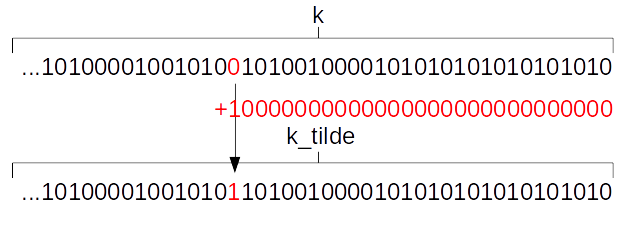
\includegraphics[width=1.0\textwidth]{img/attack2bit.png} \\
\caption{\label{f_etichetta}Attack2 with a positive injected bit fault }
\end{figure}

\begin{figure}[H]
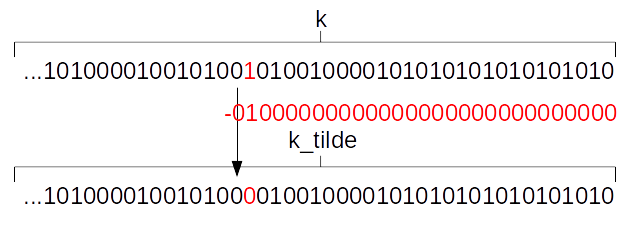
\includegraphics[width=1.0\textwidth]{img/attack2bitneg.png} \\
\caption{\label{f_etichetta}Attack2 with a negative injected bit fault }
\end{figure}

\begin{figure}[H]
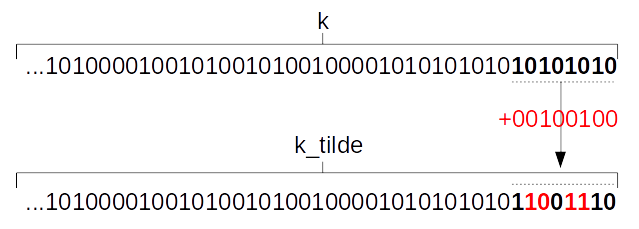
\includegraphics[width=1.0\textwidth]{img/attack2byte.png} \\
\caption{\label{f_etichetta}Attack2 with a positive injected byte fault }
\end{figure}

\begin{figure}[H]
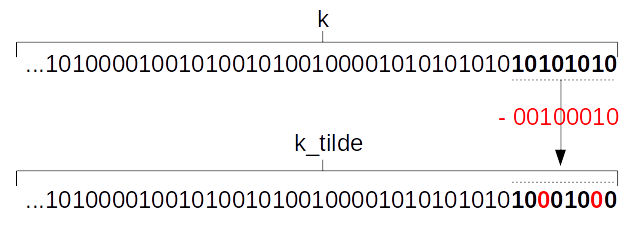
\includegraphics[width=1.0\textwidth]{img/attack2byteneg.png} \\
\caption{\label{f_etichetta}Attack2 with a negative injected byte fault }
\end{figure}


\paragraph{Bit level fault}

The attacks with an injected bit fault proceeds as follows: 
\begin{itemize}
\item Obtain the correct signature $s = k^{-1}(m + xr) $
\item Obtain the faulty signature $\tilde{s} = \tilde{k}^{-1}(m + xr)$
\item Notice that \\\\$\frac{s}{\tilde{s}}  = \frac{k^{-1}(m+xr)}{\tilde{k}^{-1}(m+xr)}$

\item In case of a positive fault $k+2^{i} $ we have \\\\$\frac{s}{\tilde{s}} = \frac{k^{-1}(m+xr)}{(k+2^{i})^{-1}(m+xr)}$

\item In case of a negative fault $k-2^{i} $ we have\\\\ $\frac{s}{\tilde{s}} = \frac{k^{-1}(m+xr)}{(k-2^{i})^{-1}(m+xr)}$

\item calulating k for both the case we have: \\\\$k_{faultpos} = \frac{\tilde{s}2^{i}}{s-\tilde{s}}$ \\
$k_{faultneg} = \frac{\tilde{s}2^{i}}{\tilde{s}-s}$ 

\item After having calculated k, we can derive the private key x as:\\\\ $x = \frac{sk - m}{r}$


\end{itemize}

Notice that in this case we need the value of \textit{k} in order to calculate \textit{x}.Obviously we don't have it a priori, but we can discover it trying to bruteforce the exponent \textit{i} of 2 in the formula $k_{faultpos} = \frac{\tilde{s}2^{i}}{s-\tilde{s}}$,so basically we calculate k for every possible \textit{i} such that 0<=i<=qbits and we try to derive \textit{x} employing the just calculated \textit{k} with the formula $x = \frac{sk - m}{r}$, finally if our correctness check it's succesfull we can conclude that was the correct \textit{k} and so this is the correct private key \textit{x} calculated, otherwise we try with another \textit{i} and restart.

\begin{algorithm}[H]
  \KwData{A message \textit{m}, the correct signature <r,s> , the faulty signature <r,$\tilde{s}$>}
  \KwResult{The private key \textit{x} of the dsa key pair employed to sign the message \textit{m}}
  
  i=0\;
  
  //\textit{trying all the possibilities for positive faults}\;
  \While{i $<=$ qbits}{
  $k_{faultpos} = \frac{\tilde{s}2^{i}}{s-\tilde{s}}$\;
  $x = \frac{sk - m}{r}$\;
  \eIf{correctness-check(x)==True}{print "dDSA private key cracked!"\;return 1\;}{ i++\;continue\;}
  }

  i=0\;  
  
  //\textit{trying all the possibilities for negative faults}\;
  \While{i $<=$ qbits}{
  $k_{faultneg} = \frac{\tilde{s}2^{i}}{\tilde{s}-s}$ \;
  $x = \frac{sk - m}{r}$\;
  \eIf{correctness-check(x)==True}{print "dDSA private key cracked!"\;return 1\;}{ i++\;continue\;}
  }
  
  print "Something went wrong"\;
  return -1

  \caption{Attack 2, bit level}
\end{algorithm}

The complexity of the algorithm is O(2n) where n=qbits. 

\paragraph{Byte level fault}

The attacks with a byte fault proceeds as follows: 
\begin{itemize}
\item Obtain the correct signature $s = k^{-1}(m + xr) $
\item Obtain the faulty signature $\tilde{s} = \tilde{k}^{-1}(m + xr)$
\item Notice that \\\\$\frac{s}{\tilde{s}}  = \frac{k^{-1}(m+xr)}{\tilde{k}^{-1}(m+xr)}$

\item In case of a negative fault $k-b2^{i} $ we have\\\\ $\frac{s}{\tilde{s}} = \frac{k^{-1}(m+xr)}{(k-b2^{i})^{-1}(m+xr)}$

\item In case of a positive fault $k+b2^{i} $ we have \\\\$\frac{s}{\tilde{s}} = \frac{k^{-1}(m+xr)}{(k+b2^{i})^{-1}(m+xr)}$


\item calulating k for both the case we have: \\\\$k_{faultpos} = \frac{\tilde{s}b2^{i}}{s-\tilde{s}}$ \\
$k_{faultneg} = \frac{\tilde{s}b2^{i}}{\tilde{s}-s}$ \\

\item After discovered the k, we can calculate the private key x as:\\\\ $x = \frac{sk - m}{r}$

Notice that in this case, as before, we need a bruteforce in order to discover the right \textit{b} and \textit{i} ( which byte has been flipped, 0<=i<=qbits and the value of the fault b, 0<=b<=255) and so to finally calculate \textit{k}. The index \textit{i} is the value of the shift of the fault value b (we are trying all the possible value, for all the possible shift).

\begin{algorithm}[H]
  \KwData{A message \textit{m}, the correct signature <r,s> , the faulty signature <r,$\tilde{s}$>}
  \KwResult{The private key \textit{x} of the dsa key pair employed to sign the message \textit{m}}
  
  
  i=0\;
  b=0\;
  
  //\textit{trying all the possibilities for positive faults}\;
  \While{i $<=$ qbits}{
  \While{b $<=$ 255}{
  $k_{faultpos} = \frac{\tilde{s}b2^{i}}{s-\tilde{s}}$\;
  $x = \frac{sk - m}{r}$\;
  \eIf{correctness-check(x)==True}{print "dDSA private key cracked!"\;return 1\;}{ b++\;continue\;}
  }
  b=0\;
  i++\;  
  }

  i=0\;  
  b=0\;
  
  //\textit{trying all the possibilities for negative faults}\;
  \While{i $<=$ qbits}{
  \While{b $<=$ 255}{
  $k_{faultneg} = \frac{\tilde{s}b2^{i}}{\tilde{s}-s}$\;
  $x = \frac{sk - m}{r}$\;
  \eIf{correctness-check(x)==True}{print "dDSA private key cracked!"\;return 1\;}{ b++\;continue\;}
  }
  b=0\;
  i++\;  
  }
  print "Something went wrong"\;
  return -1

  \caption{Attack 2, byte level}
\end{algorithm}
\end{itemize}

The complexity of the algorithm is O(2 \cdot 255 \cdot n) where n=qbits.

\subsection{Generalizing the fault model}
During the explanation of the attack 2 we said that we considered only two injection models: the bit level and the byte level, but since often you can't control precisely where the injected fault will finish, a fault can be spread in a position larger than a byte, for example can be at WORD level, DWORD level, or at the QWORD level. 

\begin{figure}[H]
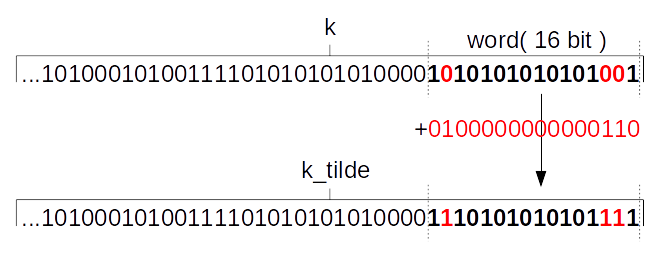
\includegraphics[width=1.0\textwidth]{img/attack2word.png} \\
\caption{\label{f_etichetta}Attack2 with a positive injected word fault }
\end{figure}

The algorithm for the attack remains the same, but in this case the nested loop described in the algorithm-4 at lines 5 and 23, will be: \textit{while b <= $2^_{16}$} and since qbits depends on the length of the key we have a complexity of O($2^_{16}$ \cdot qbits). With the longest key size considered (p=3072,q=256) we will have a number of iteration of $2^_{16}$ \cdot $2^{8} = 2^_{24}$; in order to compute this we would need a better parallelized algorithm using a framework like OpenCL\cite{opencl}.

The same thing applies to the DWORD level (32 bit) and the QWORD level (64 bit) the first will have a max. number of iteration of: $2^_{32}$ \cdot $2^{8} = 2^_{40}$, the latter will have a max. number of iteration of: $2^_{64}$ \cdot $2^{8} = 2^_{72}$.

\begin{figure}[H]
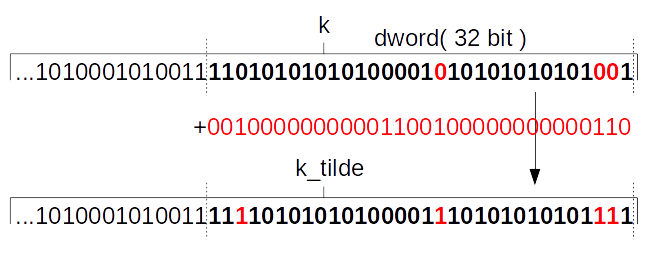
\includegraphics[width=1.0\textwidth]{img/attack2dword.png} \\
\caption{\label{f_etichetta}Attack2 with a positive injected dword fault }
\end{figure}

Notice that a fault injected at QWORD level is the max. that we can handle, in fact handling a wider fault will require inside our attack's algorithm a number of iteration greater that $2^_{80}$ that is unfeasible; by the way a fault at the byte/WORD level is good and feasible.\\\\
Finally we can say that if we have a fault that had hitten two bits that can't be grouped in a byte/WORD/DWORD/QWORD our attack2 is not feasible, but as said before the injection of a fault at WORD level is usually feasible; If we can't inject a fault that we can handle we can in any case switch to attack1 since it doesn't need this step as explained previously.

\begin{figure}[H]
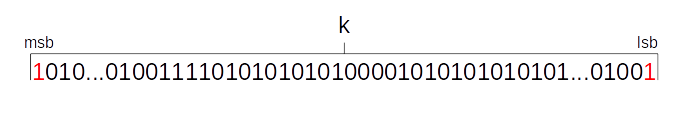
\includegraphics[width=1.0\textwidth]{img/attackfail.png} \\
\caption{\label{f_etichetta}Attack2 will fail in these cases }
\end{figure}

\section{Experimental results}
We have tested these attacks using an Intel i5 and 2GB ram with Xubuntu 14.04. 
The implementation of the DDSA algorithm as specified in the RFC\cite{rfc} is taken from the libgcrypt library version 1.6.4 \cite{lib}.\\
In order to test the attacks you have to copy our file dsa.c inside the folder /libgcrypt/cipher/ and the recompile the whole library.
\\The experiments are performed against 4 key length (expressed in the form pbits|qbits): 1024|160 , 2048|224 , 2048|256 , 3072|256.\\


For the attack 2, during the fault injection, we have to consider a completely random fault that range from an optimal case to the worst possible case.( As explained before this model is not necessary for the attack 1 because its success is independent from where the fault happens )

\begin{itemize}
\item optimal case: the fault happens on the LS[Bit/Byte] of \textit{k}; in this case we are lucky and we have the fastest possible cracking.


\begin{figure}[H]
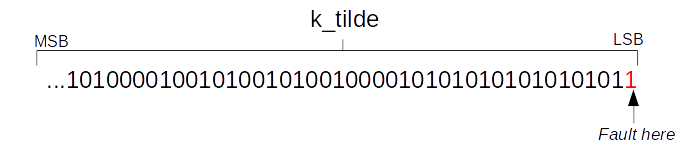
\includegraphics[width=1.0\textwidth]{img/bestcasebitfault.png} \\
\caption{\label{f_etichetta}Attack2, bit level with the best scenario }
\end{figure}

\begin{figure}[H]
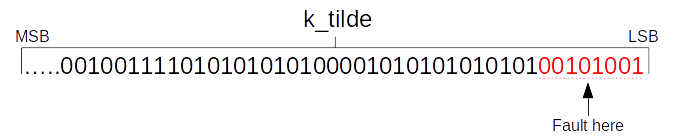
\includegraphics[width=1.0\textwidth]{img/attack2bestbyte.png} \\
\caption{\label{f_etichetta}Attack2, byte level with the best scenario }
\end{figure}


\item worst case: the fault happens on the MS[Bit/Byte] of \textit{k}; in this case we are not lucky during the fault injection and we have the slowest possible cracking.
\end{itemize}

\begin{figure}[H]
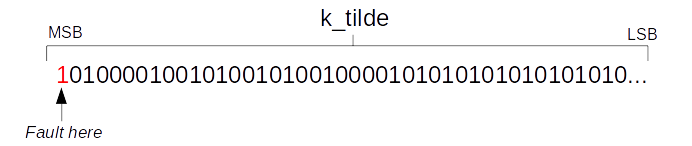
\includegraphics[width=1.0\textwidth]{img/worstcasebitfault.png} \\
\caption{\label{f_etichetta}Attack2, bit level with the worst scenario }
\end{figure}

\begin{figure}[H]
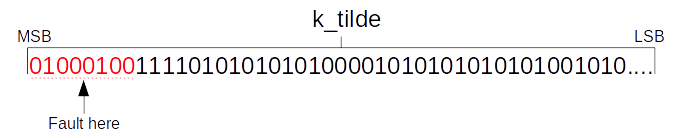
\includegraphics[width=1.0\textwidth]{img/attack2byteworst.png} \\
\caption{\label{f_etichetta}Attack2, byte level with the worst scenario }
\end{figure}

For this reason the attack's time estimated with a single run would be an imprecise measure.In order to give a better estimation of the attack's time we have randomized in the library code where the fault happen and taken the average time produced by 30 attack's rounds.The registered times include also the generation of the original signature and the validation step of the attack.

\subsection{Damage the exponentation}

In this attack the distinction between bit/byte/WORD/DWORD/QWORD level has no meaning because the time complexity is always O(1) regardless the type of the fault injected. 
\\
These are the average times necessary in order to complete the attacks,for each key length:


\begin{table}[H]
\caption{ Average times over 30 runs registered for attack 1 }
\begin{center}
\begin{tabular}{l*{6}{c}r}
Key length        & Time [ms] \\
\hline
1024/160 &       7 \\
2048/224 &       11  \\
2048/256 &       12  \\
3072/256 &       23  \\ 
\end{tabular}
\end{center}
\end{table}



\subsection{Damage the signature composition}

These are the time necessary in order to complete the attack at the bit level and byte level.
\\

\begin{table}[H]
\caption{Average times over 30 runs registered for attack 2 at the bit level}
\begin{center}
\begin{tabular}{l*{6}{c}r}
Key length        & Time [ms] \\
\hline
1024/160 &      171  \\
2048/224 &      572   \\
2048/256 &      779  \\
3072/256 &      2094  $\mathtt{\sim}$ 2 sec. \\ 
\end{tabular}
\end{center}
\end{table}


\begin{table}[H]
\caption{Average times over 30 runs registered for attack 2 at the byte level}
\begin{center}
\begin{tabular}{l*{6}{c}r}
Key length        & Time [ms] \\
\hline
1024/160 &        44267  $\mathtt{\sim}$ 44 sec. \\
2048/224 &       212596  $\mathtt{\sim}$ 3.5 min.\\
2048/256 &       8398991  $\mathtt{\sim}$ 2.20 hour. \\
3072/256 &       19778534  $\mathtt{\sim}$ 5.4 hour. \\
\end{tabular}
\end{center}
\end{table}


\section{Limits}
As presented before, in order to work the attacks presented need the parameters \textit{r} and \textit{s} from the two signatures ( the correct one and the faulty one ) of the same message \textit{m}; all this parameters are sent in plain over the untrusted channel. 
The attacks fail if any of the previous condition aren't satisfied: we can't retreive the parameter \textit{r} or \textit{s}, we can't retreive the message \textit{m}, or we can't sign the message \textit{m} two times.\\\\
Given that, a possible mitigation of these attack would be, for example, to protect the signature sended over the channel, or the  message sent, or why not both, with the public key of the destination; in this scenario we can't retreive enough parameters in order to satisfy the equations that calculate the private key.


\section{Conclusion}
According to the RFC\cite{rfc}, "the determinism of the algorithm described in this note may be useful to an attacker in some forms of side-channel attacks". With this paper we prove this fact by simulating two active side channel attacks via software that can retreive the private keys of a dsa key pair with any length. The descriptions of these attacks can be easily applied to a real scenario where the attacked system doesn't implement good countermeasures against side-channel attacks. Finally we proposed a possible easy mitigation against these attacks.

\addcontentsline{toc}{section}{\refname}
\begin{thebibliography}{10}
\bibitem{rfc} \url{https://tools.ietf.org/html/rfc6979}
\bibitem{fips} \url{http://nvlpubs.nist.gov/nistpubs/FIPS/NIST.FIPS.186-4.pdf}
\bibitem{lib} \url{https://www.gnu.org/software/libgcrypt/}
\bibitem{sexp} \url{http://rosettacode.org/wiki/S-Expressions}
\bibitem{opencl} \url{https://www.khronos.org/opencl/}
\bibitem{wiki} \url{https://en.wikipedia.org/wiki/Digital_signature}
\end{thebibliography}

\end{document}
